% Chapter 1

\chapter{Recherche d'image par le contenu} % Main chapter title

%\label{Chapter1} % For referencing the chapter elsewhere, use \ref{Chapter1} 

%\lhead{Chapter 1. \emph{Recherche d'image par le contenue}} % This is for the header on each page - perhaps a shortened title

%----------------------------------------------------------------------------------------

\section{Introduction}

	La recherche d'image par le contenu (Content Based Image Retrieval - CBIR) est le concept de chercher une image dans une large collection d'image et les extraire sans l'ajout de métadonnées. En effet, certaines méthodes de recherche d'image (par exemple: recherche par texte) dépendent en l'ajout d'annotation (mot clé, titre, ou description) à l'image. Ces méthodes dépendent en la qualité de l'annotation qui se doit  de couvrir tous les termes désirés. Cette tache peut être difficile et coûteuse ou même encore infaisable quand la collection d'image est trop large.

\begin{figure}[htbp]
	\centering
		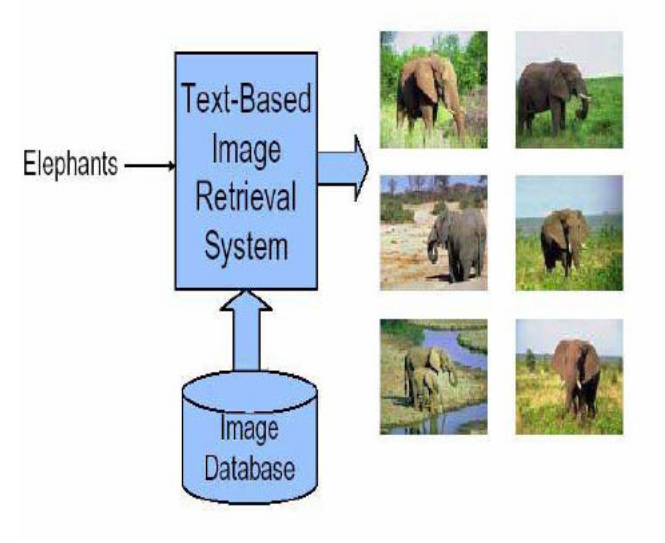
\includegraphics[width=3.5in]{Figures/textBasedIR.png}
	\caption[An Electron]{Recherche d'image par texte [Mee and Sus 13]}
	\label{fig:Electron}
\end{figure}

	Pour faire face à ce problème, d'autres techniques basées sur le contenu des images ont été développées, et qui font appel à deux domaines de recherches :

\textbf{Gestion de base de données:} Optimisation des méthodes de stockages, d'indexation multidimensionnel et du temps de réponse.

\textbf{Vision artificielle:} Représentation et extraction des caractéristiques des images.


\begin{figure}[H]
	\centering
		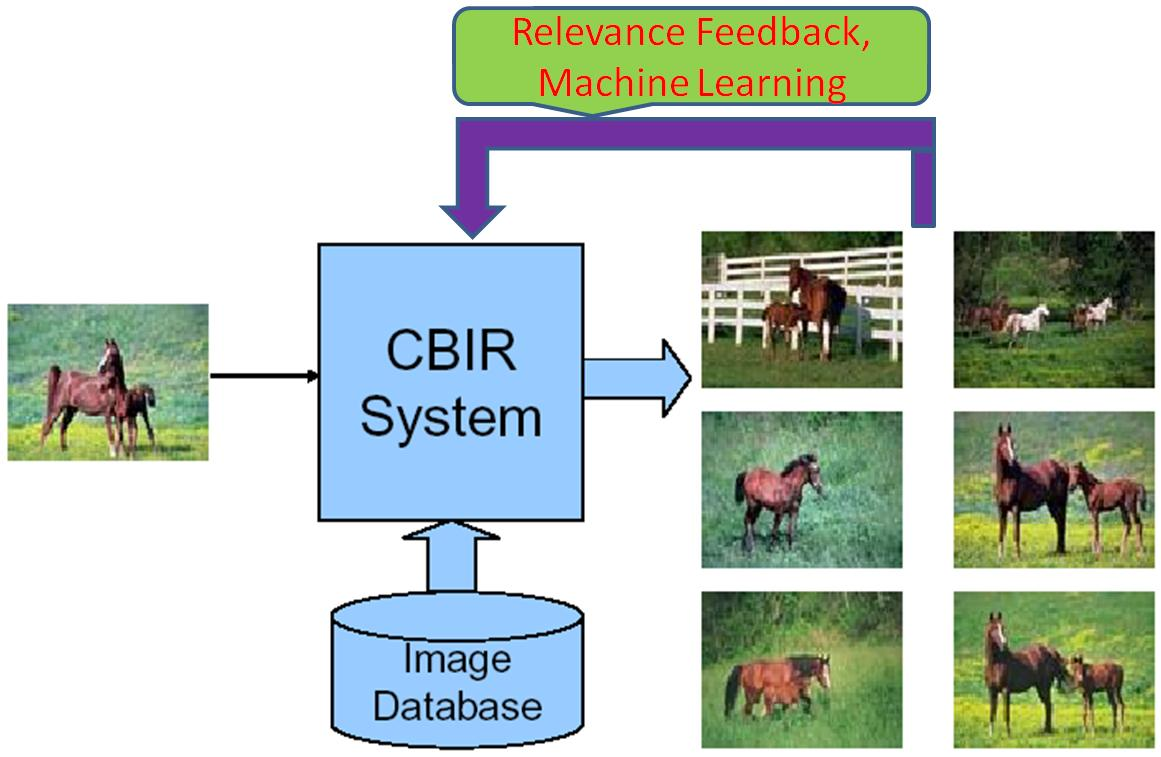
\includegraphics[width=3.5in]{Figures/cbir.JPG}
	\caption[An Electron]{Recherche d'image par le contenu [Mee and Sus 13]}
	\label{fig:Electron}
\end{figure}


\section{La conception d'un CBIR}

Les systèmes de recherches d'images par contenu sont généralement basés sur des caractéristiques prédéfinies qui sont:

\textbf{Descripteur  de couleur:} Grâce à  leurs représentations compactes et de faible complexité, la comparaison directe des histogrammes de couleur est communément utilisée.
\textbf{Descripteur de texture:} Matrice de co-occurence, Local Binary Pattern (LBP) [2]
\textbf{Descripteur de forme:} Descripteur de Fourier et moment invariants.
Et plus récemment, des descripteurs locaux tel que le SIFT sont utilisés.

\section{Calcule de similarité}
	Généralement, des fonction rigides de calcule de distance comme la distance euclidienne ou la similarité basée sur le cosinus sont utilisées pour la recherche de ressemblance entre les caractéristiques extraites.

	Par-contre, ces fonctions de calcul de distance et de similarité ne sont pas toujours optimaux pour la tache complexe de recherche par contenu sur des images, et ce du au problème du “gap sémantique” entre les caractéristiques bas niveau extraite par l'ordinateur et le haut niveau de perception humaine.

	De ce fait, récemment, de grand efforts ont été fournis dans la recherche de différentes méthodes de calcul de similarité en utilisant les techniques de l'apprentissage automatique.  Parmi ces dernières, des travaux se sont concentrés sur l'apprentissage de hachage ou code compacte. Des propositions ont été faites pour des méthodes d'apprentissage de MAPPING de données de hautes dimensions vers des codes binaires qui préservent la similarité sémantique.  [Sin and Ans 15]

\section{Types de CBIR}

	Quatre approches conceptuelles différentes ont été développées [Sin and Ans 15]:

\subsection{Basée-région :} Le Netra et Blobworld sont deux anciens systèmes de recherche d'images basés régions [6]. Pendant la recherche, un utilisateur est fourni avec des régions segmentées de l'image requête, et il est nécessaire d'attribuer plusieurs propriétés, telles que les régions à mettre en correspondance, les caractéristiques des régions, et même le poids des caractéristiques différentes [7].

\subsection{Basée-objets :} Les systèmes de récupération d'image basés sur les objets récupèrent des images à partir d'une base de données basée sur l'apparence des objets physiques dans ces images. Ces objets peuvent être des éléphants, des panneaux d'arrêt, des hélicoptères, des bâtiments, des visages, ou tout autre objet que l'utilisateur souhaite trouver. Une façon courante pour rechercher des objets dans les images est d'abord de segmenter l'image dans la base de données puis de comparer chaque région segmentée avec une région d'une certaine image requête présentée par l'utilisateur [8]. Ces systèmes de récupération d'image sont généralement couronnée de succès pour les objets qui peuvent être facilement séparés de l'arrière-plan et qui ont des couleurs distinctives ou des textures.

\subsection{Basée-exemples :} Nous nous intéresserons dans nos approches à cette catégorie qui sera détaillé dans le troisième chapitre. Les utilisateurs donnent une image d'échantillon, ou une partie d'une image, que le système utilise comme base pour le système recherche. Le système trouve ensuite les images qui sont semblables à l'image de base.

\subsection{Basée-Feedback :} Le système affiche l'utilisateur un échantillon de photos et demande à l'utilisateur des les classer. En utilisant ce classement, le système de ré-exécute les requêtes et répète cela jusqu'à ce que la bonne image soit trouvée.

\section{Systèmes et applications existants}


	Les techniques de CBIR ont été utilisées dans un grand nombre d'applications telles que: le diagnostic médical, les archives photographiques, l'identification des empreintes digitales, la reconnaissance faciale et les collections d'art.


\begin{figure}[H]
	\centering
		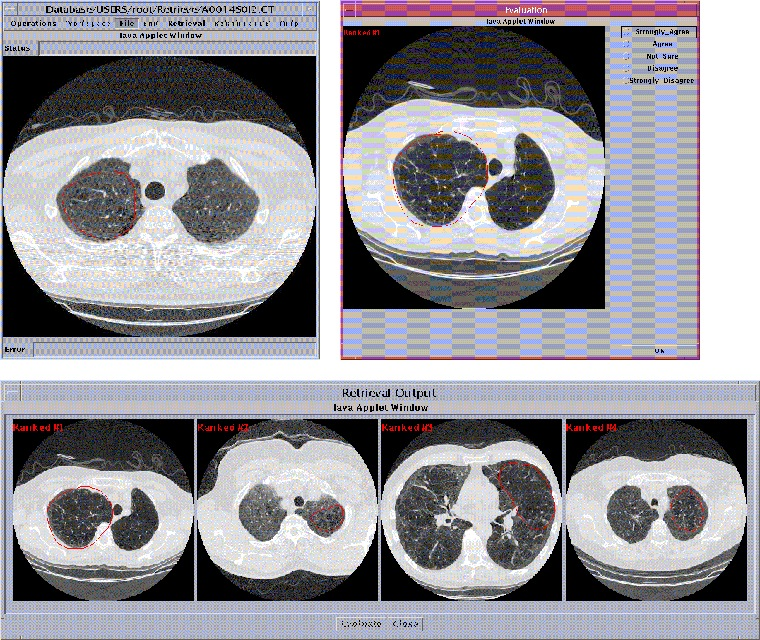
\includegraphics[width=3.5in]{Figures/cbirMedic.jpg}
	\caption[An Electron]{Application Médicale.}
	\label{fig:Electron}
\end{figure}


Fig 3. Application Médicale[4| Avinash]

Certains systèmes existants sont : 

\subsection*{QBIC}
	QBIC [6 | Niblack et tout] ou Query By Image Content, signifie requête par contenu d'image, il est le premier système de recherche d'images par le contenu commercial (CBIR). Il fournit des framework et des techniques de base pour de nombreux systèmes de récupération d'image. QBIC supporte les requêtes basée sur des exemples d'images, d'images construites par l'utilisateur et des dessins et modèles de couleur et de texture sélectionnés, etc. Les fonctions de couleur utilisées dans QBIC sont (R, G, B), (Y, i, q), ( L, a, b), et MTM (transformée mathématique Munsell), et un histogramme de couleur à k-élément. Dans son nouveau système, la recherche de texte par mot clé peut être combiné avec la recherche de similarité par contenu.



\subsection*{DigiKam}
	DigiKam est un logiciel gratuit et open-source organisateur d'image et éditeur de tag écrit en  C++. Il est une application de gestion de photos étendue construit avec des bibliothèques de KDE. Il offre, en plus de nombreuses autres fonctionnalités, les recherches inversées pour les images de la collection locale, la détection des doublons et une recherche floue par des dessins.

\subsection*{LIRE}
	LIRE est une bibliothèque Java qui fournit un moyen simple de récupérer des photos et des images en fonction de leurs caractéristiques de couleur et de texture. LIRE crée un index de Lucene des caractéristiques de l'image pour la récupération du contenu d'image basé (CBIR). Facile à utiliser, des méthodes pour rechercher l'index et les résultat sont fournies par LIRE. La bibliothèque LIRE et l'application de démo - ainsi que toutes les fichiers sources de test et de développement - sont disponibles sous la licence GNU GPL.

D'autres projets comprennent:
- The GNU Image-Finding Tool
- Google Image Search
- eBay Image Search

Une liste plus exhaustive peut être trouvée dans ce article :

$$https://en.wikipedia.org/wiki/List_of_CBIR_engines$$

\begin{figure}[H]
	\centering
		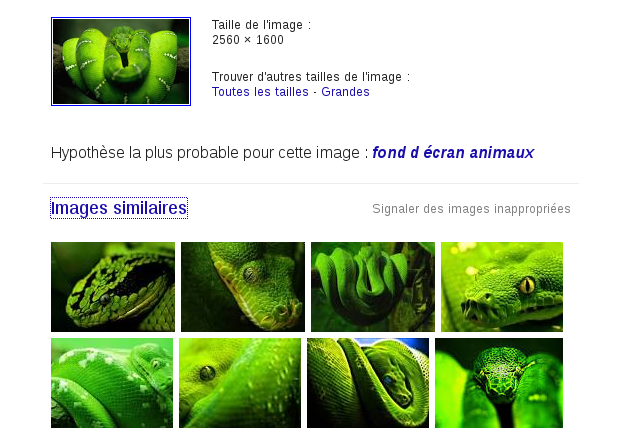
\includegraphics[width=3.5in]{Figures/googleImage2.png}
	\caption[An Electron]{Rechherche d'images de Google}
	\label{fig:Electron}
\end{figure}

\section{Problème du Semantic Gap}

	Parmi les problèmes  les plus difficiles qui font face au CBIR, nous trouvons le fossé sémantique. Il est défini comme la différence entre la faible niveau de représentation de l'information (y compris, mais pas seulement des images) dans l'ordinateur et la sémantique de haut niveau derrière elle (en d'autres mots, le sens qu'il est censé représenter).
Récemment, de nouvelles approches pour résoudre ce problème, consistent en appliquant des techniques d'apprentissage machine pour permettre à l'ordinateur de construire sa propre représentation hiérarchique d'une image au lieu de calculer les caractéristiques de manuellement.


\section{Conclusion}

